\documentclass[11pt,onecolumn]{article} %twocolumn

\usepackage{tikz}
\usepackage{esvect}
\usepackage{amsmath}
\def\checkmark{\tikz\fill[scale=0.4](0,.35) -- (.25,0) -- (1,.7) -- (.25,.15) -- cycle;} 

%opening
\title{Twitter Sentiment Analysis with Neural Networks}
\author{Pedro M. Sosa \& Shayan Sadigh}

\begin{document}
	
	\maketitle
	
	\begin{abstract}
		In recent years neural networks have become very popular in supervised learning problems and are worth looking at for anyone considering to do research in machine learning. In this exploratory paper we create our own hand-coded neural network and use it to perform sentiment classification on tweets. We also build and use a neural network using the Keras machine learning library to compare our results with. We achieve around 60\% to 70\% accuracy depending on the parameters and input representations used for the tweets.
	\end{abstract}
	
	\section{Introduction}
	Neural Networks are becoming an increasingly common approach to solve Machine Learning problems. Developments in the past decade have led neural networks to outperform other machine learning algorithms in speech recognition, recognizing human handwriting, and other tasks. This paper aims to give a solid groundwork for researchers wishing to understand and design their own Neural Networks. Furthermore, we seek to frame these explanations using real world scenarios. In this case our Neural Network's goal will be to extract sentiment analysis from Twitter data. This problem is an active problem that many companies and organizations seek to solve, since it could provide valuable marketing information, better feedback analyses, and tracking of overall client sentiment through the Twitter social media platform.
	
	\par During our research we built our own Feed-Forward Neural Network in Python and we compared it's behaviour against a similar NN built with Tensorflow \& Keras, a popular Python Machine Learning Library. Furthermore, we experimented with multiple Neural Network parameters to not only fine-tune both implementations, but to also understand their effects on the learning of the NN. Lastly we give different approaches on how to convert the twitter datasets into useful input for the NN, and we analyse how each representation affects accuracy. 
	\par It is our hope that these experiments might give other researchers a strong introduction on how NN works and how to use them to approach the Sentiment Analysis problem.
	
	
	\section{Building A FeedForward Neural Network}
	\subsection{Basics}
	
	\begin{figure}[h]
		\centering
		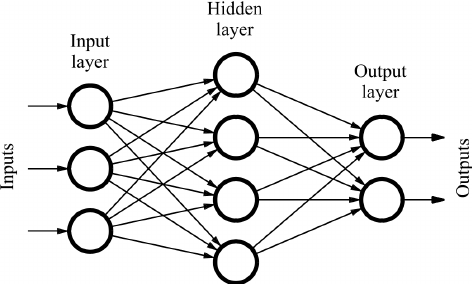
\includegraphics[scale=0.5]{images/network}
		\caption{Layout of a feedforward network, bias nodes excluded.}
	\end{figure}
	
	Like any supervised learning algorithm, a neural network is a function that takes an input and produces an output. For example, when a neural network trained for image recognition is inputted the image of a dog, the neural network could output "dog". Internally, the output is produced through a "feedforward" calculation.
	
	Feedforward neural network must be trained with labeled data in order to produce meaningful outputs. The process by which neural networks learn from labeled data is known as backpropagation.
	
	A feedforward network is made up of nodes and edges. Each node is part of a layer, and each node in a layer points to every node in the next layer. Input is fed to the first layer, the input layer. The input follows the edges to the nodes in the next layer, and so on until it reaches the output layer.
	
	Each edge is associated with a weight. When an input travels down an edge, it is multiplied by the weight associated with the edge.
	
	Each node (except for those in the input layer) takes the weighted sum of all the inputs pointing to it, plus some bias term, and is passed into an activation function. The activation function maps arbitrary numbers to a manageable range, such as between 0 and 1.
	
	
	\subsection{Forward Propagation}
	
	In a feedforward network, a node in one layer has one connection to every node in the next layer.
	
	The connections between two layers can be represented by an adjacency matrix with each entry representing an edge between two nodes in different layers. We can imagine each layer of edges in the network as a matrix of size [number of nodes in the layer, number of nodes in the next layer]. Each row represents a node in the current layer and each column represents the weight along the edge from a node in the current layer to a node in the next layer.
	
	A network with n layers can be represented by n-1 adjacency matrices, one matrix for each layer of connections between two layers of nodes.
	
	Every node is also associated with a bias term, which we can imagine as being stored in separate "bias nodes". For each layer in the network, we keep a vector b of size [number of nodes in the layer], where each entry in the vector represents a bias term associated with a node.
	
	Formally, for each layer in the network with the exception of the input layer, we calculate the following:
	
	\[ \vec{a^l} = \sigma (w^l\vec{a}^{l-1} + \vec{b^l}) \]
	
	Which means that the activation values at layer l is equal to the activation values at layer l-1 dot product with the weights connecting layers l-1 and l, each entry in the resulting vector then summed with its respective bias terms at layer l, all passed into the activation function.
	
	This process is applied to every layer in the network. The output of our network is \[a^{output\ layer}\] the activation values at the output layer.
	
	
	
	\subsection{Backpropagation}
	
	Forward propagation is the process used to calculate the output of our network given some input. Backpropagation is the process used to train our neural network given labeled data to learn from.
	
	When training our neural network we feed it (x, y) pairs, where y is the value (or vector if there's more than one output node) we want it to output when given x. First, we have our neural network make a prediction for x using forward propagation. Backpropagation then calculates the error between the prediction and actual y value and uses it to adjust the weights throughout the network in such a way that the next time the neural network performs forward propagation on x, it will predict a value a little closer to the actual value y.
	
	Here we list the formulas necessary to perform backpropagation. Curious readers can find their derivations and deeper explanations from a multitude of sources available on the internet.
	
	After running forward propagation to get the predicted output, we compute the following for every output node k in the output layer:
	
	\[ \delta_k = a_k(1-a_k)(a_k - y_k)\]
	
	Rather than iterate through each of k nodes, we can write this in vector form:
	
	\[ \vec \delta^l = \vec a^l(1-\vec a^l)(\vec a^l -\vec y^l)\]
	
	For every hidden layer l, we calculate the following:
	
	\[ \vec \delta^l = \vec a^l(1-\vec a^l)(\vec \delta^{l+1} \vec w^l)\]
	
	We adjust each layer of weights and biases by the following:
	
	\[ \Delta W^l =  -\delta^l a^{l-1}\]
	\[ \Delta b^l =  -\delta^l\]
	\[ W^l =  W^l + \Delta W^l \]
	\[ b^l =  b^l + \Delta b^l\]
	
	
	\section{Pre-processing Datasets}
	Most Neural Networks accept only numerical inputs, thus we need to find a way to represent "tweets" (strings of max. 140 characters) as numerical data. In our case, we attempted 3 different methods: Bayesian Probabilities, Word Embeddings, and Feature Vectors.
	
	\subsection{Bayesian Probabilities}
	Our first and very naive approach to representing our dataset was to convert each tweet into a vector $V=[P_{good}(W_1),P_{bad}(W_1),....,P_{good}(W_n),P_{bad}(W_n)]$ where $n \geq 70$. 
	\par In other words, the vector contained the probabilities for each single word in the tweet that such word was of positive or negative sentiment. Notice that our vectors where of size 70 (Max amount of words in a tweet) and smaller tweets would be padded with zeros.
	\par The probabilities were calculated in exactly the same way as one would using the Naive Bayes Classifier methodology. In other words:
	\begin{center}
		$P_{good}(W_i)= \frac{W_i \text{occurrences in good Dict.}}{ \text{Size of good Dict.}}$\\
		$P_{bad}(W_i)= \frac{W_i \text{occurrences in bad Dict.}}{ \text{Size of bad Dict.}}$
	\end{center}
	
	
	\subsection{Word Embeddings}
	Word embeddings is a more recent approach for word representation in which all words in a given vocabulary are plotted described as n-dimensional vectors. These vector representations have been shown to hold the relation between words  \cite{goldberg2014word2vec,mikolovword2vec}. There are multiple instances of Neural Networks that use Word Embeddings to solve text related problems  \cite{tang2014learning,maas2011learning,tang2014coooolll}. Following the previous examples, we decided to represent the words in our dataset as 32-dimensional arrays. We employed Keras' Word Embedding methods to build these vectors.
	
	\subsection{Twitter Specific Features}
	Although Word Embeddings are a very popular way to deal with text data, they are very generic and don't assume anything from the given text. However, Twitter has very particular features that distinguish it from other text forms. For example, Twitter data can contain Mentions\textit{(@user)} and Hashtags \textit{(\#topic)} that could provide very meaningful. Furthermore, Tweets are only 140 characters long, which might lead people to shorten words in unexpected ways or make more constant the use of emojis. Knowing this, we decided to also test  tweets as a feature vector.
	
	\par Our original feature vector included multiple different features that could potentially describe our dataset. We ran Correlation-based Feature Subset Selection \cite{hall1998practical} on WEKA \cite{Garner95weka} to determine which features had the most predictive ability and least redundancy. this narrowed our feature vector to use the most descriptive features. Table \#1 shows all the features tested and the ones that where ultimately selected.
	
	\begin{center}
		\begin{tabular}{ | l | l || c |}
			\hline
			Feature Name & Description & Selected \\
			\hline
			
			chwd & \# of Characters/ \# of Words & \checkmark \\
			
			exclamation & \# of exclamation marks (!) & \checkmark \\
			
			smile & \# of positive emoticons & \checkmark \\
			
			sad & \# of negative emoticons & \checkmark \\
			
			url & \# of URLs shared & \checkmark \\
			
			ellipsis & \# of ellipsis (...) & \checkmark \\
			
			mention & \# of mentions (@someone) & \checkmark \\
			
			netprob & $\sum_{W \in Tweet} (P_{pos}(W) - P_{neg}(W))$ & \checkmark\\
			
			question & \# of question marks (?) &  -\\
			
			pronoun & \# of pronouns (I, me, mine...) &  -\\
			
			hashtags & \# of hashtags (\#topic) &  -\\
			
			capitals & \# of uppercase letters &  -\\
			
			length & Length of the Tweet &  - \\
			
			\hline
		\end{tabular}
		\newline
		\newline
		\textbf{Table 1 } - List of features tested. The selected one refer to the the ones used selected through Weka and used in our experiments.
	\end{center}
	
	%\subsection{Meta Features}
	%\textbf{[TODO: Will you use meta-features such as replies, date and time, etc.]}
	
	
	
	\section{Selecting Parameters}
	Once we had built our own Neural Network and had parsed our dataset into word embeddings and feature vectors we proceeded to test different scenarios to find the best possible parameter configuration for both our NN and the Keras NN.
	\par Our initial experiments consisted on evaluating the best parameter configuration for both Neural Network. These parameters were: batch size, \# of hidden layers, size of hidden layers, and \# of epochs. 
	\begin{figure}[t]
		\centering
		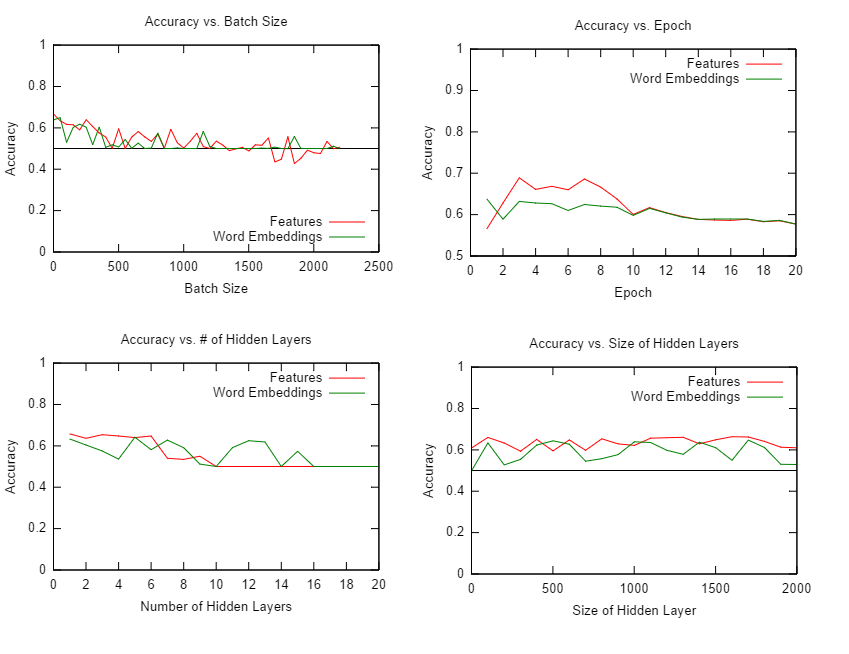
\includegraphics[width=1.0\linewidth]{images/all_in_one}
		\caption{Parameter Fine-Tuning Results for the Keras NN}
		\label{fig:all_in_one}
	\end{figure}
	
	\subsection{Batch Sizes}
	A Neural Network can be trained with batches of multiple training cases at a time. These batches (also known as minibatches) allow users to cut dataset into smaller segments, feed it through the Neural Network, and update the NN with the mean of the final calculated gradient descent.
	\par Having big batches allows the NN to learn from a big dataset faster, as the throughput of each operation is much higher. However, since the update is being done with the mean of the gradient descent of all the batch's training cases, it is possible to loose precision and over-fit to the training data.
	\par Using Keras, our experiments (Figure \ref{fig:all_in_one}) clearly show that the Keras NN performed better with batches of around 1 - 300 in size. Higher batches tended to converge to a 0.5 or worse accuracy, which could be attributed to over-fitting. We found similar results with our own Network.
	
	\subsection{\# of Hidden Layers}
	It would seem intuitive that the more layers we have the more accuracy we will obtain, since our Neural Network will have an greater ability to recognize different patterns. However, this is not the case, as we increase the number of hidden layers, we find the accuracy of our results drop drastically. This particular behavior commonly referred to as the "vanishing gradient problem"  \cite{hochreiter1998vanishing} is a typical in Neural Networks that rely on propagation and gradient-based learning.
	\par More specifically, this problem happens because during the backpropagation phase, the gradient by which a weight will be updated is calculated using the chain rule. This means that "front" layers will have exponentially smaller update gradients than the "back" layers. In other words, the front-layers train exponentially slower leading to poor results.
	\par In our particular experiments, both the Keras NN and our own NN worked best with 1-2 layers.
	
	\subsection{Size of Hidden Layers}
	While increasing the size of a single hidden layer substantially decreased computational performance, it did not seem to affect the accuracy of the NN. It is important to mention however, that having a hidden layer that was too small was actually detrimental to the performance while using Features as an input. This might be because the amount of neural paths are so limited that no real features can be distinguished. However, this threshold might be different depending on the NN. On the Keras NN, we saw chose 250 as the layer size due to good results and performance; On our own NN, we chose 20 as the layer size.
	
	\subsection{\# of Epochs and Learning Rate}
	The number of Epochs refers to the number of times an NN is trained with the same test data. Having multiple repetitions might be useful especially if you have a small training set, however too many repetitions can quickly lead to over-fitting. 
	\par The \# of epochs is directly related to the learning rate, which is the rate by which the NN corrects its weights during backpropagation. The Keras NN did not seem to allow us to change that rate and as such we found that the optimal amount of epochs was 3. However, on our own NN we allowed changes to the learning rate and as such we choose a substantially smaller rate which resulted in us having to do 100 epochs.
	
	\begin{center}
		\begin{tabular}{| c | c | c | c | c |}
			\hline
			NN & Batch Size & Epoch & Size of Hidden Layer & \# of Hidden Layers\\
			\hline
			Keras & 1 & 3 &  250 & 1 \\
			\hline
			Own & 50 & 100 &  20 & 1 \\
			\hline
		\end{tabular}
		\newline
		\newline
		\textbf{Table 2 } - Selected Parameters for both our own NN and the Keras NN.
	\end{center}
	
	
	\section{Results}
	After selecting the best parameter setup, we ran our NN and the Keras NN with both Naive Bayesian Probabilities, Word Embeddings, and Feature Vectors.
	
	
	\begin{center}
		Keras Nerual Network's Performance
		\begin{tabular}{ | c | c | c | c | c |}
			
			\hline
			Input Type & Average Acc.  & Max Acc & Min .A& Std. Dev. \\
			\hline
			Bayesian Prob. & 63.04\% & 63.82\% & 62.32\% & 0.0053 \\
			\hline
			Word Embeddings & 61.40\% &	65.05\% & 58.30\% & 0.0150 \\
			\hline
			Feature Vectors & 67.20\% & 71.15\% & 63.30\% & 0.0177 \\
			\hline
		\end{tabular}
		\newline
		\newline
		\textbf{Table 3} - Accuracy results for 100 trial runs of the Keras NN using Bayesian probabilities, Word Embeddings, or Feature Vectors as input.
	\end{center}
	
	\begin{center}
		Our Own Neural Network's Performance
		\begin{tabular}{ | c | c | c | c | c |}
			\hline
			Input Type & Average Acc.  & Max Acc & Min .A& Std. Dev. \\
			\hline
			Bayesian Prob. & 62.90\% & 63.92\% & 62.14\% & 0.0070 \\
			\hline
			Word Embeddings & 58.43\% &	61.77\% & 55.02\% & 0.0162 \\
			\hline
			Feature Vectors & 66.80\% & 68.75\% & 60.35\% & 0.0158 \\
			\hline
		\end{tabular}
		\newline
		\newline
		\textbf{Table 4} - Accuracy results for 100 trial runs of our Neural Network using Bayesian probabilities, Word Embeddings, or Feature Vectors as input.
	\end{center}
	
	\subsection{Analysing Dataset Representation}
	Our final results show that how you choose to represent your data has a significant impact on the accuracy of the NN. Notice that when we used word embeddings we obtained worse results that simply using Bayesian probabilities or our Feature Vectors. We believe this is due to nature of tweets; As we described above, tweets seem to be a particularly noise type of written data. It is the inclusion of hashtags, mentions, URLs and emojis, atypical word shortenings, typos, and other irregularities that hampers performance. On the other hand, harnessing those atypical features through our feature vector seemed to provide us with good results. 
	\par Finally it is worth noting that the results obtained using the Bayesian Probabilities as inputs were very similar to what we found when running an actual Naive Bayes Classifier on the dataset. When we ran our trial runs with Bayesian probabilities, we saw a much lower standard deviation than what we saw with the other methods. We have a hunch that our neural network essentially learns to become a Naive Bayes Classifier when we feed it these probabilities.
	
	\subsection{Keras vs. Our Own Neural Network}
	
	Our own Neural Network achieved an accuracy level quite similar to the Keras NN. Using Bayesian Probabilities and Feature Vectors it obtain average accuracy that differed by 0.3\%-0.4\% less. In the case of word embeddings it did do worse and differed by 2.97\% less.
	
	\par Further development in our own Neural Network could provide better results. For example, adding cross-entropy cost function over the quadratic cost function we've been using may have resulted in better performance, as cross-entropy is more appropriate for classification problems like this.
	
	
	\section{Further Work}
	
	While we mostly tested FeedForward Neural Networks, there are multiple variations of NNs that could provide a better solution for the Twitter Sentiment Analysis problem. There has been some studies \cite{tang2014learning,tang2014coooolll} that use Convolutional Neural Network to enhance the pattern learning from inputs described with word embeddings. As a final set of experiments we built these NNs with the Keras library and tested them using Word Embeddings as our input.
	
	\subsection{Convolutional Neural Networks}
	\begin{figure}
		\centering
		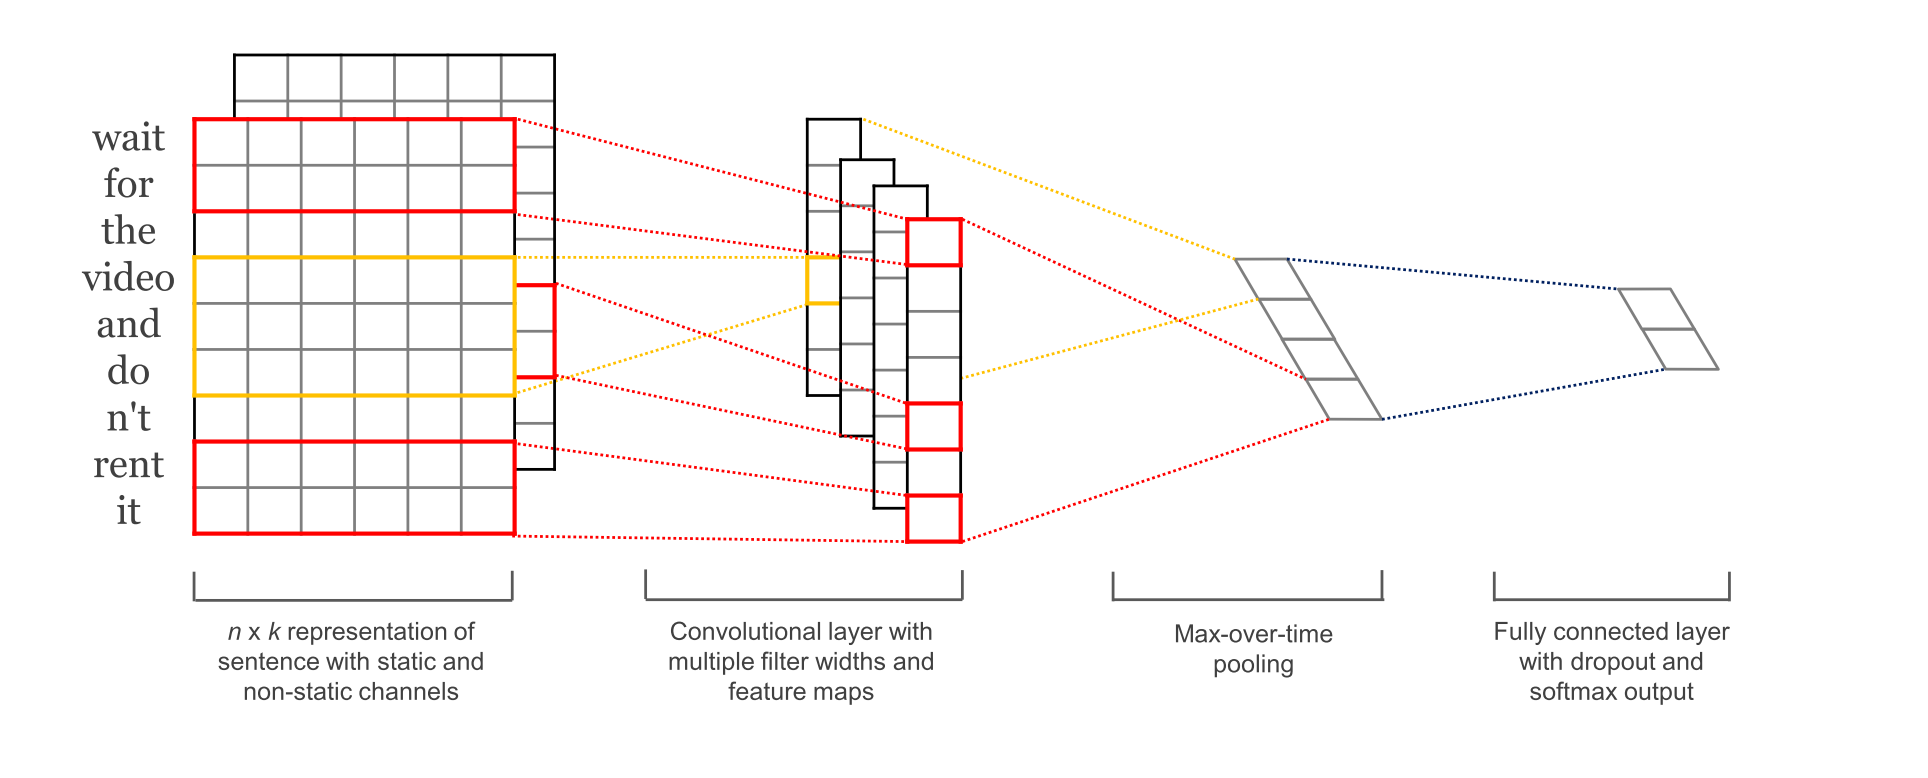
\includegraphics[width=1.0\linewidth]{images/cnn}
		\caption{Kim, Y. (2014). Convolutional Neural Networks for Sentence Classification}
	\end{figure}
	
	CNNs \cite{Kim14} have the ability to recognize repeating patterns within smaller segments of the data. This is specially important with text based problems, as it can pick up phrases or colloquialisms that other simpler NNs would miss. For example, "down to earth" is a phrase that a simple Neural Network might catch as negative, since the word "down" is more commonly used in Tweets to explain negative sentiments. However a CNN could learn that the specific combination "down to earth" is an overall positive phrase. It also has the potential of learning about double negatives and other more complicated linguistic patterns.
	\par We found that adding Convolutional layer (with a filter window size of 3 and an overall kernel size of 32) to our original NN would increase the overall accuracy by roughly 2.8\%. With more research and work in CNNs we imagine they could result in a substantial increase in accuracy.
	
	
	%\subsection{Long Short-Term Memory Recurrent Neural Network}
	%\textbf{[TODO: Brief explanation of what are LSTM Networks - perhaps a pretty picture too.]}.
	
	
	\begin{center}
		\begin{tabular}{ | c | c | c | c | c |}
			\hline
			NN Type & Average Acc. & Max Acc. & Min Acc. & Std. Dev. \\
			\hline
			Original NN & 61.40\% &	65.05\% & 58.30\% & 0.0150 \\
			\hline
			CNN & 64.21\% & 67.05\% & 62.10\% & 0.0134 \\
			\hline
			%LSTM RNN & - & - & - & - \\
			%\hline
		\end{tabular}
		\newline
		\newline
		\textbf{Table \#5} - Accuracy results for 100 trial runs of the different NN programmed with Keras and using Word Embeddings as their input.
	\end{center}
	
	
	\section{Conclusion}
	Throughout our different experiments we managed to achieve around 65\% to 70\% accuracy extracting sentiment information from Twitter data with a simple FeedForward network. We explained and implemented a basic FeedFoward Network that obtained results comparable to those of the established ML Python Library Keras. We explained the effect of different parameters configurations, possible pitfalls and solutions to obtain the most accurate results from Neural Networks. Furthermore, we show how different representations of the dataset affect the accuracy of the results.
	
	Our hope is that this work (along with the provided code found at github.com/pmsosa/CS273-Project) could provide a good groundwork for researchers who wish to understand and further engage in the area of Neural Networks and deep learning.
	
	%References
	%http://cs.ucsb.edu/~jod//papers/c-12-socialcom2013.pdf
	
	\bibliographystyle{ieeetr}
	\bibliography{main}
	\nocite{iamtrask,neuralnet}
	
\end{document}